\documentclass[10pt]{article}
\usepackage{amsmath}
\usepackage{amssymb}
\usepackage{amsthm}
\usepackage{braket}
\usepackage{hyperref}
\usepackage{setspace}
\usepackage{tikz}
\usepackage{graphicx}
\usetikzlibrary{quantikz2}

\doublespacing
\allowdisplaybreaks

\begin{document}
\section*{Introduction}
We hope to solve the equation 
\begin{align*} 
    i \partial_t \psi = (-i \sigma_x \partial_x + m \sigma_z + f(x))\psi
\end{align*}
where $\psi = (\psi_1 \psi_2)^T$, and $f$ is some potential function. In theory,
this is only slightly different from Schrödinger. If we can store the spinor $\psi$,
nearly all the same methods can be used to solve Dirac; we will use Strang splitting
to approximate the solution by solving each term individually. Note that $\propto$ can
usually be interpreted as "equal up to normalization."
\section*{Splitting}
Like in Schrödinger, we approximate the solution using splitting of the unitary transformation,
but this time we use the Strang splitting:
\begin{align*}
    \psi(x, t_{j+1}) = e^{-\partial_x \sigma_x \frac{\Delta t}{2}} e^{-i(m\sigma_z + f(x))\Delta t} e^{-\partial_x \sigma_x \frac{\Delta t}{2}} \psi(x, t_j) + O(\Delta t^3)
\end{align*}
With $\frac{t}{\Delta t}$ timesteps, this gives a second order in $\Delta t$ accumulated error 
$O(\frac{t}{\Delta t}\Delta t^3) = O(t \Delta t^2)$. Also recognize that $[m \sigma_z, f(x)I] = 0$,
so we can split exactly $e^{-i(m \sigma_z + f(x)) \Delta t} = e^{-im \sigma_z} e^{-if(x)}$. The
implementation of these operators and storage of the spinor on qubits are detailed below.
\section*{Discretization and Storage}
Fortunately, the problem of storing the spinor on qubits has a simple solution: we
maintain a register to store position, as in Schrödinger, and add one qubit as
an indicator. We discretize $\psi_1$ and $\psi_2$ into $\ket{\psi_1}$ and $\ket{\psi_2}$
as we know how from Schrödinger, and store the state $\psi$ as
\begin{align*}
    \ket{\psi} &\propto \sum_{k=0}^{N-1} \left(\psi_1(x_k)\ket{0} + \psi_2(x_k)\ket{1}\right) \otimes \ket{k} \\
               &= \ket{0} \otimes \left( \sum_{k=0}^{N-1} \psi_1(x_k) \ket{k} \right) + \ket{1} \otimes \left( \sum_{k=0}^{N-1} \psi_2(x_k) \ket{k} \right) \\
               &\propto \ket{0} \otimes \ket{\psi_1} + \ket{1} \otimes \ket{\psi_2}
\end{align*}
With the indicator as the most significant qubit, this is equivalent to concatenating the
column vectors of amplitudes for $\ket{\psi_1}$ and $\ket{\psi_2}$. Regarding measurement
probabilities, if we measure only the register storing position, and leave the indicator
qubit unmeasured, the probability of measuring $\ket{k}$ is $p(k) \propto |\psi_1(x_k, t)|^2 + |\psi_2(x_k, t)|^2$.
This is justified as follows: the state $\ket{\psi}$ has density matrix
\begin{align*}
    \ket{\psi}\bra{\psi} &\propto (\ket{0} \otimes \ket{\psi_1} + \ket{1} \otimes \ket{\psi_2})(\bra{0} \otimes \bra{\psi_1} + \bra{1}\otimes \bra{\psi_2}) \\
    &= \ket{0}\bra{0} \otimes \ket{\psi_1} \bra{\psi_1} + \ket{0}\bra{1} \otimes \ket{\psi_1} \bra{\psi_2} + \ket{1}\bra{0} \otimes \ket{\psi_2} \bra{\psi_1} + \ket{1}\bra{1} \otimes \ket{\psi_2} \bra{\psi_2}
\end{align*}
Measurement probabilities of the position register are given by the reduced density
matrix obtained by tracing out the spinor qubit. Taking the partial trace, we get
\begin{align*}
    \mathcal{\rho} &\propto \ket{\psi_1}\bra{\psi_1} + \ket{\psi_2} \bra{\psi_2} \\
                   &= \sum_{l=0}^{N-1}\sum_{j=0}^{N-1}(\psi_1(x_l)\psi_1(x_j)^* + \psi_2(x_l)\psi_2(x_j)^*) \ket{l} \bra{j}
\end{align*}
Thus the probability of measuring $\ket{k}$ at time $t$ is $p(k) = \text{tr}(\ket{k}\bra{k}\rho) 
\propto |\psi_1(x_k, t)|^2 + |\psi_2(x_k, t)|^2$ by orthonormality of the computational basis.
\section*{Transport Term}
We concern ourselves with the equation $i \partial_t \psi = -i \partial_x \sigma_x \psi$.
Recognizing that $\sigma_x = H \sigma_z H$, where, $H$ is the Hadamard matrix, this
system is equivalent to $\partial_t H \psi = -\partial_x \sigma_z H \psi$. Letting
$\varphi := (\varphi_1, \varphi_2)^T = H \psi$, since $\sigma_z$ is diagonal, the system 
is decoupled: $\partial_t \varphi = -\partial_x \sigma_z \varphi$. Equivalently,
\begin{align*}
    &\partial_t \varphi_1 = -\partial_x \varphi_1 \\
    &\partial_t \varphi_2 = \partial_x \varphi_2
\end{align*}
This is a first order linear transport equation, which has a known solution
for initial conditions $\varphi_j^0(x) = \varphi_j(x, 0)$: $\varphi_1(x, t) = \varphi_1^0(x-t)$
and $\varphi_2(x, t) = \varphi_2^0(x+t)$. For the sake of implementation on a quantum computer,
we solve using the Fourier transform $\mathcal{F}$ to get
\begin{align*}
    \varphi(x, t) =
    \begin{pmatrix}
        \mathcal{F}^{-1}(e^{-i \xi t}\mathcal{F}(\varphi_1^0)(\xi)) \\
        \mathcal{F}^{-1}(e^{i \xi t}\mathcal{F}(\varphi_2^0)(\xi)) \\
    \end{pmatrix}
\end{align*}
Hence on the quantum computer we map $\ket{s} \otimes \ket{k} \mapsto \ket{s}
\otimes (QFT e^{(-1)^{s+1} i\xi_k \Delta t} QFT^\dag \ket{k})$, where as before, $\xi_k = \frac{\pi}{L}(2k - N)$.
A new concern we have in Dirac is that any $\theta$ dependent global phase incurred in 
the application of $e^{i\theta k}$ is now a relative phase between $\varphi_1$ and $\varphi_2$
that we need to correct for. We write the phase shift operation more carefully 
with respect to global phase changes. Note that I've changed the implementation
of $e^{ik} := \bigotimes_{j=0}^{n-1} P(2^j)$ to use phase gates, rather than differences of identity and $Z$ gates.
This makes global phase easier to keep track of.
\begin{align*}
    \exp\left((-1)^{s+1} i\frac{\pi}{L}(2k-N)\Delta t\right) &= \exp\left((-1)^{s} i N \frac{\pi}{L}\Delta t\right)\exp\left((-1)^{s+1} 2i \frac{\pi}{L} \Delta t k\right) \\
    &= \exp\left((-1)^{s} i N \frac{\pi}{L}\Delta t\right)\bigotimes_{j=0}^{n-1} P\left((-1)^{s+1}2^{j+1}\frac{\pi}{L} \Delta t \right)
\end{align*}
$\varphi_1$ picks up a phase of $e^{\frac{\pi i N \Delta t}{L}}$, and $\varphi_2$ picks
up a phase of $e^{-\frac{\pi i N \Delta t}{L}}$, which we build in by applying 
$R_Z\left(\frac{-2\pi N \Delta t}{L}\right)$ to the spinor qubit. The quantum 
circuit we implement to apply the shift phase is below. $\theta = \frac{\pi}{L} \Delta t$.
\begin{center}
\makebox[\textwidth][c]{%
\begin{quantikz}[wire types={q,q,n,q,q}, row sep={0.9cm,between origins}]
    \lstick{$\ket{k_0}$} & \gate{P(2\theta)} &&&&&& \gate{P(-2\theta)}&&&  \\
    \lstick{$\ket{k_1}$} && \gate{P(4\theta)} &&&& \gate{P(-4\theta)} &&&&       \\
    \lstick{$\vdots$}    &&&&&&&&&   &\\ 
    \lstick{$\ket{k_{n-1}}$} &&& \gate{P(2^{n}\theta)} &  & \gate{P(-2^{n}\theta)} &&&& & \\
    \lstick{$\ket{s}$}   & \ctrl{-4}  & \ctrl{-3}  & \ctrl{-1}  & \gate{X} & \ctrl{-1}  & \ctrl{-3}  & \ctrl{-4}  &  \gate{X} & \gate{R_Z(-2 N \theta)} &
\end{quantikz}%
}
\end{center}
Sandwiching this with $QFT$ and $QFT^\dag$ solves the linear transport equation,
which is certainly interesting on its own, so I have included a plot below of a
solution with two Gaussians $\varphi_1$ and $\varphi_2$.
\begin{center}
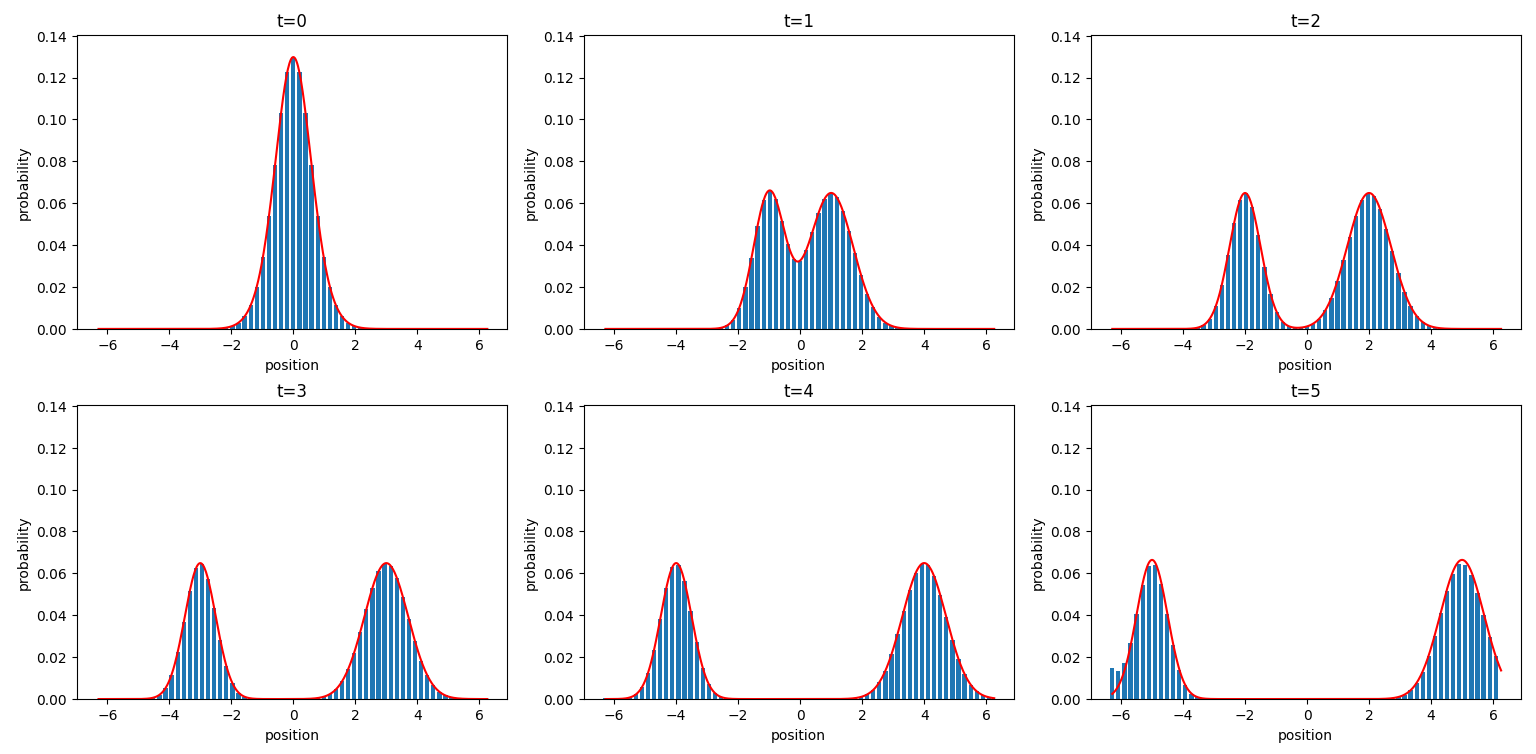
\includegraphics[scale=0.4]{../plots/transport.png}
\end{center}
As interesting as this is, our concern is with Dirac, and still we need to be able
to map between $\ket{\psi}$ and $\ket{\varphi}$. This is fortunately very simple and
reveals itself after a bit of algebra. Recalling that $\psi = H\varphi$ and $\varphi = H \psi$,
and we have the state $\ket{\varphi} \propto \ket{0}\ket{\varphi_1} + \ket{1}{\ket{\varphi_2}}$
\begin{align*}
    \ket{\psi} &\propto \ket{0}\ket{\psi_1} + \ket{1} \ket{\psi_2} \\
               &= \frac{\ket{0}}{\sqrt{2}}\left(\ket{\varphi_1} + \ket{\varphi_2}\right) + \frac{\ket{1}}{\sqrt{2}}\left(\ket{\varphi_1} - \ket{\varphi_2}\right) \\
               &= \frac{\ket{0} + \ket{1}}{\sqrt{2}}\ket{\varphi_1} + \frac{\ket{0} - \ket{1}}{\sqrt{2}}\ket{\varphi_2} \\
               &= (H \otimes I)\ket{\varphi}
\end{align*}
The same gate maps both directions, so we can transform between $\ket{\varphi}$ and $\ket{\psi}$
with a Hadamard gate on the spinor qubit. Thus our solution to $\partial_t \psi = -\sigma_x \partial_x \psi$
is given by simply applying $H$ to the spinor qubit, following the work above for the linear transport,
then applying another $H$. This is the circuit returned by transport().
\section*{Mass Term}
We now concern ourselves with the mass term $i \partial_t \psi = m \sigma_z \psi$.
Fortunately, $\sigma_z$ is diagonal in the standard basis, so we have the following solution.
\begin{align*}
    \psi(x, t) = 
    \begin{pmatrix}
        e^{-imt}\psi_1^0(x) \\
        e^{imt}\psi_2^0(x)
    \end{pmatrix}
\end{align*}
On qubits we want to map $\ket{0}\ket{\psi_1} + \ket{1}\ket{\psi_2} \mapsto e^{-im \Delta t}
\ket{0} \ket{\psi_1} + e^{im \Delta t}\ket{1}\ket{\psi_2}$. This is implemented with
a single $R_Z(2m \Delta t)$ on the spinor qubit.
\section*{Potentials}
We implement a linear potential and the quantum harmonic oscillator potential,
giving a phase gate decomposition here.
For $f(x) = x$, the Trotter term we implement is
\begin{align*}
    \psi(x, t) = e^{-ixt} \psi_0(x)
\end{align*}
on qubits, this looks like
\begin{align*}
    e^{-if(x)\Delta t}: \ket{k} &\mapsto e^{-ix_k\Delta t} \ket{k} \\
    &= e^{id\Delta t} e^{-ik\Delta x \Delta t} \ket{k} \\
    &= \prod_{j=0}^{n-1} e^{-i2^jk_j \Delta x \Delta t} \text{\quad up to global phase}
\end{align*}
Hence up to global phase, this potential is given by $\bigotimes_{j=0}^{n-1} P(-2^j \Delta x \Delta t)$
on the position register. For the quantum harmonic oscillator, we have already
derived a working circuit using RZ gates, but for completeness here is a derivation
for the implementation in dirac.py, decomposing the operation with phase gates.
We want to implement $e^{-i x_k^2 \Delta t} = e^{-i (-d + k \Delta x)^2 \Delta t}$,
which is given by $e^{2idk\Delta x \Delta t}e^{-ik^2 \Delta x^2 \Delta t}$ up to global phase.
The first term in the product is linear in $k$, so we know already by previous work
how to decompose such a thing into phase gates. Considering the $e^{-ik^2}$ term, we have
\begin{align*}
    e^{-ik^2} &= e^{-i\left( \sum_{j=0}^{n-1} 2^j k_j \right) \left( \sum_{l=0}^{n-1} 2^l k_l \right)} \\
    &= e^{\sum_{j=0}^{n-1} \sum_{l=0}^{n-1} 2^{j+l} k_j k_l} \\
    &= e^{\sum_{j=0}^{n=1} 2^{2j}k_j} e^{\sum_{j=0}^{n-1}\sum_{l=0}^{n-1}2^{j+l+1}k_j k_l}
\end{align*}
This can be decomposed into phase gates as follows.
\begin{align*}
    e^{-ik^2} &= \prod_{j=0}^{n-1} P_j(-2^{2j})\prod_{l=j+1}^{n-1}CP_{jl}(-2^{j+l+1})
\end{align*}
Finally deriving our quantum circuit for $f(x) = x^2$, we have
\begin{align*}
    e^{-if(x_k)\Delta t} &= \prod_{j=0}^{n-1} P_j(2^{j+1}d \Delta x \Delta t)P(-2^{2j}\Delta x^2 \Delta t)
    \prod_{l=j+1}^{n-1} CP_{jl}(-2^{j+l+1}\Delta x^2 \Delta t) \\
    &= \prod_{j=0}^{n-1} P_j(2^j \Delta x \Delta t(2d - 2^j \Delta x)) \prod_{l=j+1}^{n-1}CP_{jl}(-2^{j+l+1}\Delta x^2 \Delta t)
\end{align*}
\section*{Testing}
Here I justify a test of the transport term. By our previous work,
we know $\psi = H \varphi$, thus the initial condition $\varphi^0$ is given by 
\begin{align*}
    \varphi^0 = H \psi^0 = 
    \frac{1}{\sqrt{2}}
    \begin{pmatrix}
        \psi_1^0 + \psi_2^0 \\
        \psi_1^0 - \psi_2^0
    \end{pmatrix}
\end{align*}
Solving now for $\psi$,
\begin{align*}
    \psi(x, t) &= H \varphi(x, t) \\
    &= \frac{1}{\sqrt{2}}
    \begin{pmatrix}
        \varphi_1(x, t) + \varphi_2(x, t) \\
        \varphi_1(x, t) - \varphi_2(x, t)
    \end{pmatrix} \\
    &= \frac{1}{\sqrt{2}}
    \begin{pmatrix}
        \varphi_1^0(x - t) + \varphi_2^0(x + t) \\
        \varphi_1^0(x - t) + \varphi_2^0(x + t) \\
    \end{pmatrix} \\
    &= \frac{1}{2}
    \begin{pmatrix}
        \psi_1^0(x-t) + \psi_2^0(x-t) + \psi_1^0(x+t) - \psi_2^0(x+t) \\
        \psi_1^0(x-t) + \psi_2^0(x-t) - \psi_1^0(x+t) + \psi_2^0(x+t) \\
    \end{pmatrix}
\end{align*}
Thus from any initial condition $\psi^0$, we can construct exact solutions according
to the scheme above and discretize on qubits as $\ket{\psi_\text{ideal}}$. If our
true $\ket{\psi}$ is successfully computed up to a global phase, we should have
$|\braket{\psi|\psi_{\text{ideal}}}| = 1$. Defining the error $\varepsilon :=
\left|1 - |\braket{\psi|\psi_{\text{ideal}}}|\right|$, we can say the test passes if $\varepsilon$
is smaller than some predefined tolerance. Testing the mass term is much easier;
since the system is already uncoupled, we can solve
\begin{align*}
    i \partial_t \psi = m \sigma_z \psi \implies \psi(x, t) =
    \begin{pmatrix}
        e^{-im t} \psi_1^0(x) \\
        e^{imt} \psi_2^0(x)
    \end{pmatrix}
\end{align*}
and test by the same procedure.

\end{document}
